%\documentclass[twoside]{pwrthesis}
\documentclass[twoside]{iisthesis}
% ---
\usepackage{polski}
\usepackage[utf8]{inputenc}
\usepackage{amsmath}
\usepackage{tocloft}
\usepackage{listings}
\usepackage{algorithm}
\usepackage{algorithmic}
\usepackage{subcaption}
\usepackage{mathtools}
\usepackage{graphicx}
\usepackage[colorinlistoftodos]{todonotes}
\usepackage{url}
\usepackage{pgfplots, pgfplotstable}
\selectlanguage{polish}
% Dodane przeze mnie d
\usepackage{fancyvrb} % dla srodowiska Verbatim
\usepackage{color}
\usepackage{lscape}

\hypersetup{
    colorlinks,
    linkcolor={black!50!black},
    citecolor={black!50!black},
    urlcolor={black!80!black}
}

\definecolor{gray}{rgb}{0.4,0.4,0.4}
\definecolor{darkblue}{rgb}{0.0,0.0,0.6}
\definecolor{cyan}{rgb}{0.0,0.6,0.6}

\lstset{
  basicstyle=\ttfamily,
  columns=fullflexible,
  showstringspaces=false,
  commentstyle=\color{gray}\upshape
}

\lstdefinelanguage{XML}
{
  morestring=[b]",
  morestring=[s]{>}{<},
  morecomment=[s]{<?}{?>},
  stringstyle=\color{black},
  identifierstyle=\color{darkblue},
  keywordstyle=\color{cyan},
  morekeywords={xmlns,version,type}% list your attributes here
}

\lstset{
  language=XML,
   literate={ć}{{\'c}}1
}
\renewcommand*{\lstlistingname}{Kod źródłowy}
% definicje kolorow
\definecolor{ciemnoSzary}{rgb}{0.15,0.15,0.15}
\definecolor{szary}{rgb}{0.5,0.5,0.5}
\definecolor{jasnoSzary}{rgb}{0.2,0.2,0.2}

% Konfiguracja verbatima
\fvset{
	frame=single,
	numbers=left,
	fontsize=\footnotesize,
	numbersep=12pt,
%	framerule=.5mm,
	rulecolor=\color{ciemnoSzary},
%	fillcolor=\color{jasnoSzary},
	framesep=4pt,
	stepnumber=1,
	numberblanklines=false,
	tabsize=2,
%	formatcom=\color{szary}
}
\newcommand{\listequationsname}{Spis wzorów}
\newcommand{\equationcaption}[1]{\begin{flushright}\emph{#1}\end{flushright}}
\newcommand{\rightcaption}[1]{\begin{flushright}\emph{#1}\end{flushright}}
\newlistof{myequations}{equ}{\listequationsname}
\newcommand{\myequations}[1]{%
\addcontentsline{equ}{myequations}{\protect\numberline{\theequation}#1}\par}

\newcommand{\listofmyalgorithmsname}{Spis algorytmów}
\newlistof{myalgorithm}{algo}{\listofmyalgorithmsname}
\newcommand{\myalgorithm}[1]{%
\addcontentsline{algo}{myalgorithm}{\protect\numberline{\thealgorithm}#1}\par}


\newcommand{\listofmyfiguresname}{Spis rysunków}
\newlistof{myfigure}{figu}{\listofmyfiguresname}
\newcommand{\myfigure}[1]{%
\addcontentsline{figu}{myfigure}{\protect\numberline{\thefigure}#1}\par}

\floatname{algorithm}{Algorytm}

\newtheorem{mydef}{Definicja}



\begin{document}


\newcommand{\resultChart}[7][140]{
\def\dataS{{#2}}
	\begin{figure}[H]
	
\centering

\begin{center}
\begin{tikzpicture}
 
\begin{axis}[
ybar,
bar width=20,
legend style={at={(0.5,-0.25)},
anchor=north,legend columns=-1},
ylabel={Wartość miary},
symbolic x coords={\dataS},
xtick=data,
height=  {#1},
width=0.8\textwidth,
ymin=0, ytick={0,0.5,1},
ymax=1.5,
nodes near coords,
nodes near coords align={vertical},
]
\addplot coordinates { (\dataS,{#3}) };
\addplot coordinates {(\dataS,{#4}) };
\addplot coordinates { (\dataS,{#5}) };
\legend{Recall,Precission,F1-Score}
\end{axis}
\end{tikzpicture}
\end{center}
\caption{{#6}}
\myfigure{{#6}}
\label{{#7}}
\end{figure}
}


\pgfkeys{/pgf/number format/use comma}
\pgfkeys{/pgf/number format/.cd, set thousands separator={}}%
\nocite{*}
\title{ Wielokryterialny problem rozmieszczenia zraszaczy wodnych na zadanej powierzchni }
\titleEN{ Multicriteria water sprinklers deployment problem on a given area}
\shortTitle{SHORT TITLE}
\author{inż. Grzegorz Dziedzic}
\advisor{dr Mariusz Fraś}
\instituteLogo{logos/pwr}
\slowaKluczowe{optymalizacja wielokryterialna,\\ algorytmy genetyczne,\\zraszacze wodne}

\date{\number\the\year}

% Wstawienie abstractu pracy
	%\input {abstract}

\abstractSH{SHORT ABSTRACT}

\abstractPL{
	ABSTRACT PL
}
\abstractEN{
	ABSTRACT EN
}

\maketitle

\textpages


\graphicspath{ {img/} }
\DeclareGraphicsExtensions{.pdf,.png,.jpg}
\chapter{Wstęp}
\section{Wprowadzenie}
Odpowiednie nawodnienie ogrodu jest jedną z podstawowych czynności pielęgnacyjnych. Gdy właściciel dysponuje odpowiednim budżetem najlepszym rozwiązaniem będzie dla niego inwestycja w automatyczny system nawadniania. System taki składa się z zraszaczy wodnych, rur pomiędzy nimi oraz systemu sterowania. Takie rozwiązanie pozwala zaoszczędzić czas tracony na ręcznym podlewaniu ogrodu oraz zapewnia równomierne nawodnienie na całej ustalonej powierzchni. Jednym z głównych problemów koniecznych do rozwiązania podczas instalacji takiego systemu jest odpowiednie rozmieszczenie poszczególnych zraszaczy. Te najczęściej znajdują się pod ziemią oraz posiadają wynurzalną głowicę. Z tego powodu raz zainstalowany zraszacz najczęściej zostaje na swoim miejscu, aż do momentu wymiany całej instalacji wodnej. Biorąc to pod uwagę rozmieszczenie zraszaczy powinno być dobrze przemyślane już podczas etapu projektowania systemu nawadniania. Projektując taki system należy przyjąć jako cel nawodnienie całości wskazanego obszaru jak najmniejszym kosztem przy przestrzeganiu wskazanych przez właściciela ograniczeń.

Proces projektowania sieci zraszaczy może być żmudny oraz długotrwały, biorąc pod uwagę różnorodność sprzętu dostępnego na rynku czy chociażby nieregularność powierzchni, która ma zostać nawodniona. Z pomocą może przyjść tutaj nowoczesna technologia. Opisany powyżej problem idealnie nadaje się do rozwiązania przy pomocy dostępnych algorytmów optymalizacyjnych. Praca ta będzie skupiać się na rozwiązaniu omówionego problemu poprzez opracowanie systemu wspomagania decyzji i implementację oraz porównanie wielokryterialnych algorytmów genetycznych.

\section{Cel pracy}
Opracowanie informatycznego systemu wspomagania podejmowania decyzji w rozmieszczeniu zraszaczy wodnych na zadanej powierzchni, a w szczególności zaproponowanie oraz przebadanie wielokryterialnych algorytmów genetycznych w kontekście wybranego problemu.

\section{Przegląd literatury}
Problem przedstawiony w temacie pracy nie był do tej pory poruszany w literaturze. Nie mniej jednak biorąc pod uwagę, opisane później, założenia przyjęte podczas realizacji pracy można znaleźć publikacje o tematyce zbliżonej, czyli takie w których autorzy starają się rozwiązać problem pokrycia danego obszaru (Area Coverage Problem).

W większości znalezionych publikacji do rozwiązania stawianego problemu używane są algorytmy ewolucyjne, w tym głównie algorytmy genetyczne.
Przykładem jest "REF", gdzie autorzy rozwiązują optymalizacyjny problem rozmieszczenia sensorów w sieci bezprzewodowej przy użyciu algorytmu genetycznego NSGA-II. Autorzy skupiają się na pokryciu określonego terenu sygnałem z jak najmniejszej ilości sensorów. Przedstawione wyniki są obiecujące - w 500 pokoleń ilość potrzebnych sensorów z BEGIN spadła do END.
TODO

\section{Opis pracy}
W kolejnych rozdziałach opisane będą poszczególne zagadnienia związane z realizacją celu pracy. Najpierw dokładniej opisany zostanie problem nawodnienia obszaru, czyli problem z którym muszą zmagać się wszyscy projektanci ogrodów i systemów nawadniania. Następnie wyjaśnione zostaną pojęcia optymalizacji oraz optymalizacji wielokryterialnej, czyli dwa zagadnienia na których bazuje cała praca. W kolejnym rozdziale opisane zostaną algorytmy genetyczne, zarówno te w wersji podstawowej jak i wielokryterialnej wraz z ich wybranymi wersjami, tak aby przybliżyć czytelnikowi dlaczego i w jaki sposób one działają. W następnej kolejności zostanie wyjaśnione czym jest system wspomagania decyzji, jakie założenia powinien spełniać oraz jakimi funkcjonalnościami się wyróżniać. Kolejne rozdziały będą już odzwierciedleniem wykonanej pracy i dokładnym opisem przyjętego sposobu realizacji zadania. Najpierw dokładnie opisany zostanie opracowany system wspomagania decyzji. Zaprezentowana będzie architektura oraz przykładowe zrzuty ekranu pokazujące przygotowany interfejs graficzny. W kolejnym rozdziale skonkretyzowany zostanie problem optymalizacji. Przedstawiony będzie opracowany model matematyczny, przykładowe rezultaty oraz wyniki badań mające na celu porównania wybranych wersji algorytmów genetycznych. Na końcu pracy znajdzie się podsumowanie oceniające przedstawione rozwiązanie oraz propozycje dalszego rozwoju opracowanego systemu oraz badań.

\chapter{Problem nawodnienia obszaru}
Jednym z podstawowych problemów z jakim spotykają się właściciele ogrodów jest instalacja odpowiedniego systemu nawadniania. Mogą to zrobić sami albo zlecić zadanie firmie zajmujacej się projektowaniem ogrodów i systemów nawadniania.
Jest kilka szczególnie ważnych elementów, na które należy zwrócić uwagę projektując taki system:
\begin{itemize}
	\item Odpowiedni pomiar terenu, który ma zostać nawodniony
	\item Wzięcie pod uwagę ukształtowania terenu
	\item Obliczenie potrzebnego ciśnienia wody
	\item Wybór i rozmieszczenie zraszaczy
	\item Wybór i poprowadzenie rur
	\item Umiejscowienie zaworów
\end{itemize}
Wszystkie wymienione powyżej elementy znacząca wpływają na cenę, jakość oraz wydajność zaprojektowanego systemu.\\
W tej pracy autor skupia się na dwóch z powyższych punktów: wyborze i rozmieszczeniu zraszaczy oraz poprowadzeniu rur i nie będzie brał pod uwagę reszty wymienionych punktów.\\
Odpowiednie rozmieszczenie zraszaczy jest ważne, ponieważ zapewnia równomierne nawodnienia.

\chapter{Optymalizacja}
\section{Optymalizacja jednokryterialna}
\section{Optymalizacja wielokryterialna}

\chapter{Algorytmy genetyczne}
Problem optymalizacyjny opisany na wstępie pracy został rozwiązany przy użyciu algorytmów genetycznych. Są to algorytmy, których działanie oparte jest na tych samych zasadach na których odbywa się proces ewolucji zachodzący w naturze. W tym rozdziale przedstawiony zostanie opis ogólny algorytmu genetycznego, jego powiązanie z procesami zachodzącymi w przyrodzie, schemat działania oraz dokładny opis wykorzystywanych operatorów: krzyżowania, selekcji oraz mutacji. Następnie przedstawiony zostanie koncept wielokryterialnych algorytmów genetycznych oraz opisane zostaną dwa algorytmy wykorzystane do rozwiązania przedstawionego wcześniej problemu: NSGA-II oraz SPEA.
\section{Opis ogólny}
Algorytmy genetyczne są procedurami wykorzystywanymi do rozwiązywania problemów optymalizacyjnych, opartymi o genetykę oraz selekcję naturalną. Cały proces działania takiego algorytmu można porównywać do procesu ewolucji występującego w przyrodzie. Obserwując taki proces można zauważyć, że najlepiej przystosowane osobniki mają największe szanse na reprodukcję, a więc przekazanie swojego DNA kolejnym pokoleniom. Dzieje się tak dlatego, że z punktu widzenia biologii najlepiej przystosowane osobniki to te najbardziej atrakcyjne dla potencjalnych partnerów oraz w przypadku zwierząt stadnych, te dominujące całą resztę, a więc mające pierwszeństwo jeśli chodzi o wybór partnerów, reprodukcję czy chociażby pożywianie się. Generalizując natura dąży do tego, aby do puli z której utworzone ma zostać kolejne pokolenie danej populacji trafiały jak najlepsze geny. Gdyby działo się inaczej żaden gatunek nie przetrwałby więcej niż kilkudziesięciu pokoleń.\\
Jak zostało wspomniane największe szanse na potomstwo mają osobniki najlepsze patrząc z perspektywy szansy na przetrwanie. Potomstwo par takich osobników powstaje na wskutek procesu nazywanego krzyżowaniem. Krzyżowanie polega na łączeniu genów jednego osobnika z drugim, tworząc w ten sposób potomka, charakteryzującego się cechami zarówno pierwszego jak i drugiego rodzica. Oczywiście im lepiej rodzice danego osobnika byli przystosowani, tym większa szansa, że również i on będzie stał wysoko w hierarchii.\\
Kolejnym istotnym elementem w procesie ewolucji jest mutacja. Mutacja jest losowym procesem polegającym na zmianie fragmentu kodu DNA. Poprzez taką zmianę osobnik staje się jeszcze lepiej lub gorzej przystosowany. W pierwszym przypadku jego szanse na reprodukcję wzrastają, więc jest większe prawdopodobieństwo, że zmiana wprowadzona przez mutację zostanie przekazana dalej. W drugim przypadku linia osobników ze zmienionym DNA prawdopodobnie wygaśnie zdecydowanie szybciej niż w przypadku pierwszym.

Podsumowując, proces ewolucji złożony jest z trzech elementów: selekcji, krzyżowania oraz mutacji. Na tych samych operacjach opiera się działanie algorytmu genetycznego. W kontekście algorytmu są one nazywane operatorami genetycznymi. Na rysunku \eqref{fig:ga_sequence} przedstawiony został ogólny schemat działania takiego algorytmu.
\begin{figure}[!htb]
	\makebox[\textwidth]{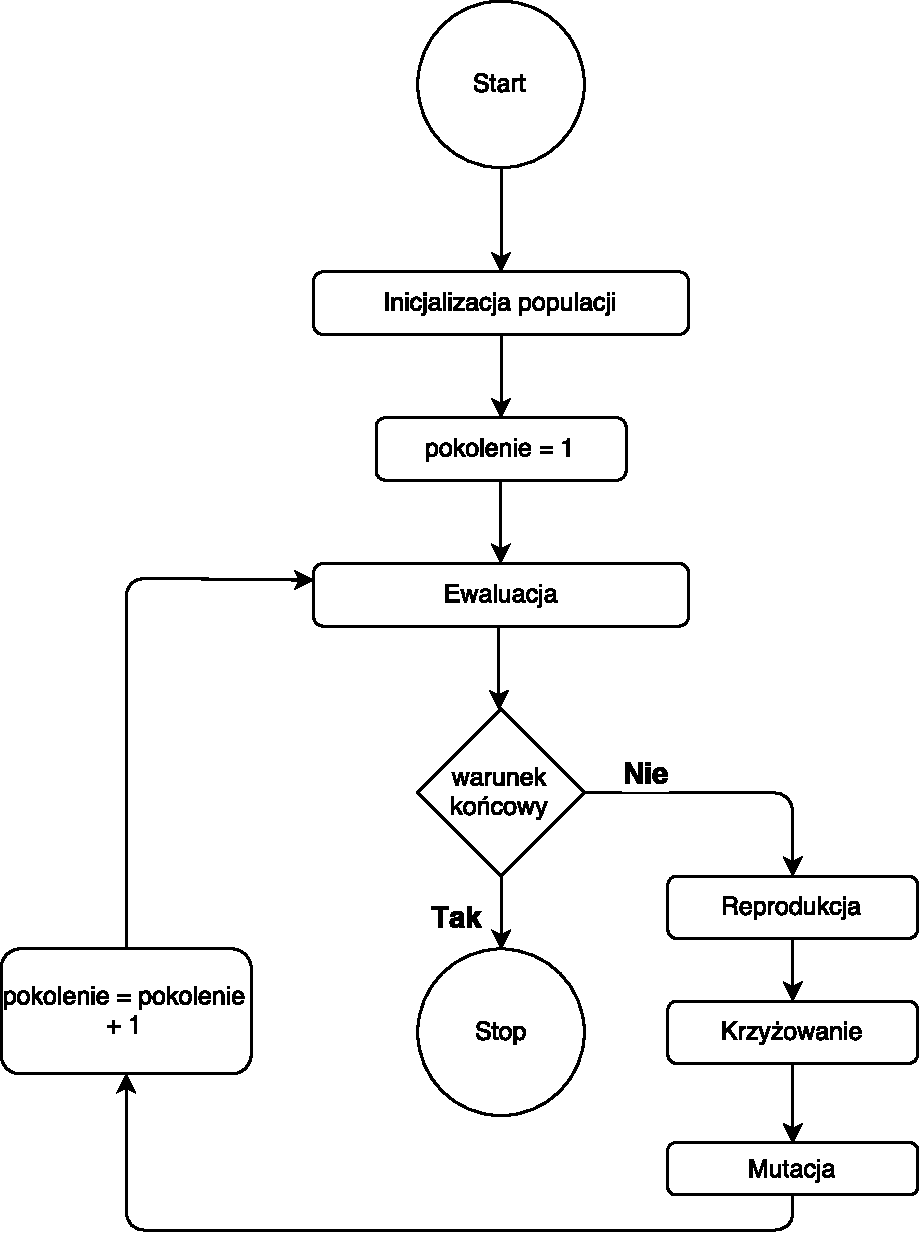
\includegraphics[ clip, scale=0.5]{ga_sequence}}
	\centering
	\caption{Schemat działania algorytmu genetycznego}
	\label{fig:ga_sequence}
\end{figure}

Punktem startowym jest utworzenie losowej populacji osobników. Następnie każdy osobnik jest oceniany przez pryzmat ustalonego kryterium. Na podstawie oceny przeprowadzany jest proces selekcji, czyli wyboru najlepszych osobników, które wykorzystane zostaną do reprodukcji. Podczas procesu reprodukcji generowane są nowe osobniki tworzące kolejne pokolenie. Każdy nowy osobnik jest wynikiem krzyżowania, czyli łączenia chromosomu dwóch rodziców w jeden. Chromosom z punktu widzenia biologii jest formą organizacji materiału genetycznego. Z punktu widzenia algorytmu będzie to zestaw parametrów charakteryzujących danego osobnika, który zostanie opisany później. Następnie chromosomy nowych osobników mogą ulec mutacji, czyli losowej zmianie pojedynczych genów. Gdy zostanie utworzona odpowiednia liczba nowych osobników, czyli powstanie nowe pokolenie, cały proces zaczyna się od początku, dopóki nie osiągnięte zostanie zdefiniowane kryterium końcowe.\\\\
W powyższym opisie pojawiło się kilka pojęć wartych wyjaśnienia.
\subsubsection{Populacja}
Populacja jest grupą o ustalonym rozmiarze. Elementami grupy są pojedyncze osobniki. Jedną z przewag algorytmów genetycznych nad tradycyjnymi technikami optymalizacyjnymi jest właśnie operowanie nie na jednym konkretnym rozwiązaniu, lecz na całej grupie. Duża różnorodność osobników w połączeniu z odpowiednim użyciem operatorów genetycznych pozwala uniknąć problemu utknięcia na optimum lokalnym.
\subsubsection{Chromosom}
Chromosom, jak zostało już wspomniane, jest sposobem reprezentacji właściwości cechujących danego osobnika. Chromosom można zdefiniować na dwa sposoby: za pomocą ciągu binarnego lub wartości rzeczywistych. Ciąg binarny jest ciągiem wartości $0$ lub $1$ ułożonych w taki sposób aby odpowiednio zakodować przekazywaną informację. W ramach przykładu załóżmy, że mamy dany cylinder o średnicy $d = 10 cm$ oraz wysokości $h = 14 cm$. Rysunek \eqref{fig:cylinder} pokazuje przykładowy sposób reprezentacji takiego cylindra w formie ciągu binarnego. 
\begin{figure}[!htb]
	\makebox[\textwidth]{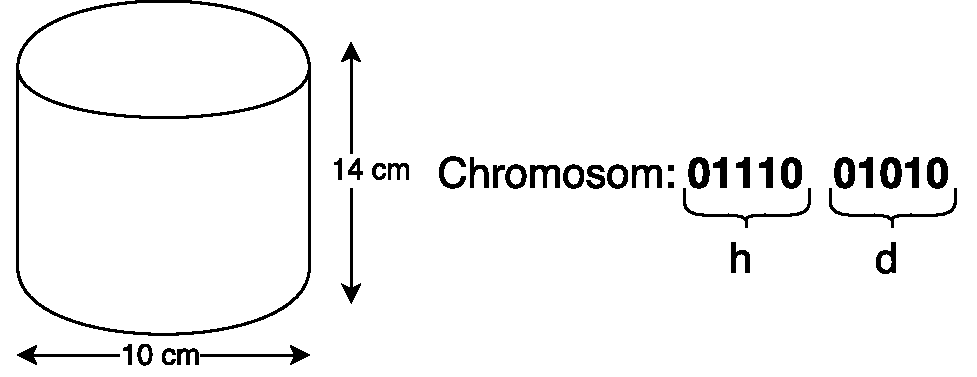
\includegraphics[ clip, scale=0.5]{cylinder}}
	\centering
	\caption{Przykład ciągu binarnego}
	\label{fig:cylinder}
\end{figure}
\\Chromosom reprezentujący cylinder złożony jest z 10 bitów. Na pierwszych pięciu z nich zakodowana jest informacja o wysokości, a na kolejnych informacja o średnicy. Wartości przedstawione przez poszczególne części ciągu należy traktować jak liczby binarne i w ten sam sposób je interpretować.

W większości przypadków preferowane jest używanie ciągu binarnego jako sposobu reprezentacji osobników. Jednym z powodów jest łatwość przeprowadzania operacji krzyżowania oraz mutacji, o których mowa będzie później. Używając reprezentacji binarnej można w prosty sposób zmienić sposób kodowania osobników bez konieczności ingerowania w operatory genetyczne - operatory krzyżowania oraz mutacji nie biorą pod uwagę sposobu w jaki informacja została zapisana w chromosomie. Kolejne argumenty przemawiające za użyciem takiej reprezentacji przedstawione zostały w pracach Hollanda (1991)REF oraz Goldberga (1993)REF. Kolejne etapy działania algorytmów genetycznych wyjaśnione zostaną przy założeniu, że osobniki przedstawione są za pomocą ciągów binarnych.
\subsubsection{Ewaluacja}
Po ustaleniu sposobu reprezentacji osobników należy wygenerować losową populację oraz poddać ją ocenie, czyli ewaluacji. Proces ewaluacji polega na przypisaniu każdemu osobnikowi odpowiedniej wartości pozwalającej ocenić go na tle reszty populacji. Korzystając z wcześniejszego przykładu załóżmy, że podczas procesu ewaluacji zdefiniowanemu wcześniej cylindrowi przypisywany jest koszt wyprodukowania, wyrażony następującym wzorem:
\begin{equation}
f(d,h) = c\big{(}\dfrac{\pi d^{2}}{2} + \pi dh\big{)}
\end{equation}
, gdzie $c$ oznacza koszt materiału na $cm^{2}$.\\
Zgodnie z podanymi wcześniej danymi oraz przy założeniu, ze $c = 0.01$ koszt wyprodukowania danego cylindra wynosi:
\[f(10, 14) = 6\]
Zakładając, że celem procesu optymalizacji jest minimalizacja kosztu wyprodukowania cylindra, należy zauważyć, że osobnik z przypisaną mniejszą wartością jest lepszy w kontekście wybranego kryterium.
\subsubsection{Reprodukcja}
Kolejnym etapem działania algorytmu genetycznego jest reprodukcja inaczej zwana też selekcją. Jest to proces mający na celu zwiększenie liczby dobrych osobników w populacji oraz redukcję liczby tych gorszych, jednocześnie utrzymując niezmieniony rozmiar całej populacji. Jest to osiągane poprzez realizację następujących zadań:\\
\begin{enumerate}
	\item Zidentyfikowanie dobrych (ocenionych powyżej średniej) osobników.
	\item Utworzenie kopii dobrych osobników.
	\item Eliminacja osobników gorszych, tak aby kopie dobrych mogły zostać dodane do populacji.\\
\end{enumerate}
Powyższe zadania mogą zostać osiągnięte przy użyciu kilku metod. Najpopularniejszymi z nich są: metoda turniejowa, metoda ruletki oraz metoda rankingu.
Metoda turniejowa polega na rozgrywaniu turniejów pomiędzy kilkoma osobnikami wybranymi losowo z populacji. Zwycięzca każdego turnieju, jako rodzic, przechodzi do etapu krzyżowania, który zostanie opisany później\eqref{fig:tournament}. Rozmiar pojedynczego turnieju znacząco wpływa na przebieg procesu selekcji. Im jest większy, tym mniejsza szansa, że słabsze osobniki przejdą do kolejnego etapu. Wbrew pozorom takie zachowanie nie jest pożądane ze względu na potrzebę zachowania różnorodności populacji. Im rozmiar jest większy tym większa szansa, że do kolejnego etapu dostanie się zbyt dużo słabszych osobników, co również nie jest dobrym rozwiązaniem. Jeśli rozmiar turnieju $S = 1$ selekcja staje się równoważna losowemu wyborowi osobnika. Najczęściej stosuje się turnieje o rozmiarze 2. Metoda turniejowa jest jedną z najczęściej wybieranych metod selekcji. Jest prosta w implementacji oraz pozwala na łatwe manipulowanie rozmiarem turnieju, co z kolei wpływa na szybkość zbliżania się znalezionych rozwiązań do rozwiązania optymalnego. Ponadto jak zostało udowodnione selekcja turniejowa zawsze zapewnia lepszą lub taką samą szybkość zbliżania się do rozwiązań optymalnych jak inne metody selekcji oraz mniejszą lub taką samą złożoność obliczeniową. Z wymienionych powyżej powodów to właśnie metoda turniejowa została zaimplementowana w wybranych przez autora algorytmach.
\begin{figure}[!htb]
	\makebox[\textwidth]{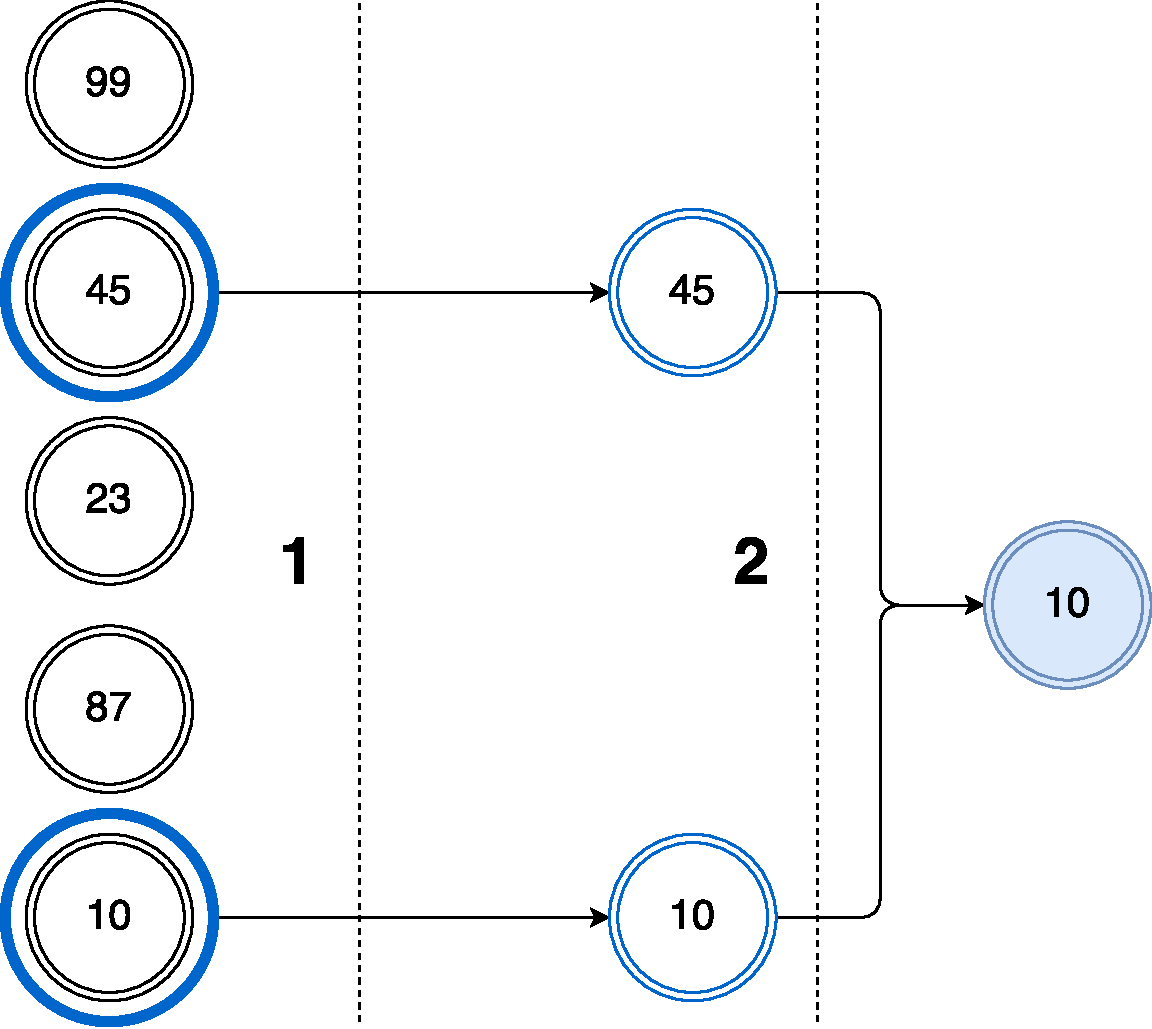
\includegraphics[ clip, scale=0.5]{tournament}}
	\centering
	\caption{Przykład rozegranego turnieju o rozmiarze 2.\\1.Wybór losowych osobników; 2.Turniej pomiędzy wybranymi osobnikami.}
	\label{fig:tournament}
\end{figure}
\section{Algorytmy wielokryterialne}
\subsection{NSGA-II}y
\subsection{SPEA}
\section{Strojenie}

\chapter{Systemy wspomagania decyzji}

\chapter{Rozwiązanie problemu}
\section{System wspomagania decyzji}
\subsection{Architektura}
\subsection{Interakcja z użytkownikiem}
\section{Optymalizacja}
\subsection{Model matematyczny}
Załóżmy, że $P$ jest wielokątem odwzorowującym kształt terenu, który ma zostać nawodniony. Poprzez opisanie danego wielokąta prostokątem otrzymujemy teren roboczy $A$. Szerokość i wysokość tego terenu są dodatkowo powiększone o największy możliwy zasięg zraszaczy, tak aby umożliwić odpowiednie sprawdzenie stopnia naruszenia ograniczeń, o których mowa później. $A$ jest dodatkowo podzielony na $m \times n$ kwadratów tworząc macierz $M$ przedstawioną na rysunku REF. Każdy element macierzy może przyjmować wartości od 0 do $ms$, gdzie $ms$ jest maksymalną liczbą zraszaczy. Wartość 0 oznacza, że dany kwadrat nie został podlany. Wartość większa od 0 mówi o tym przez ile zraszaczy dany obszar został nawodniony.

%\begin{figure}[!htb]
%	\makebox[\textwidth]{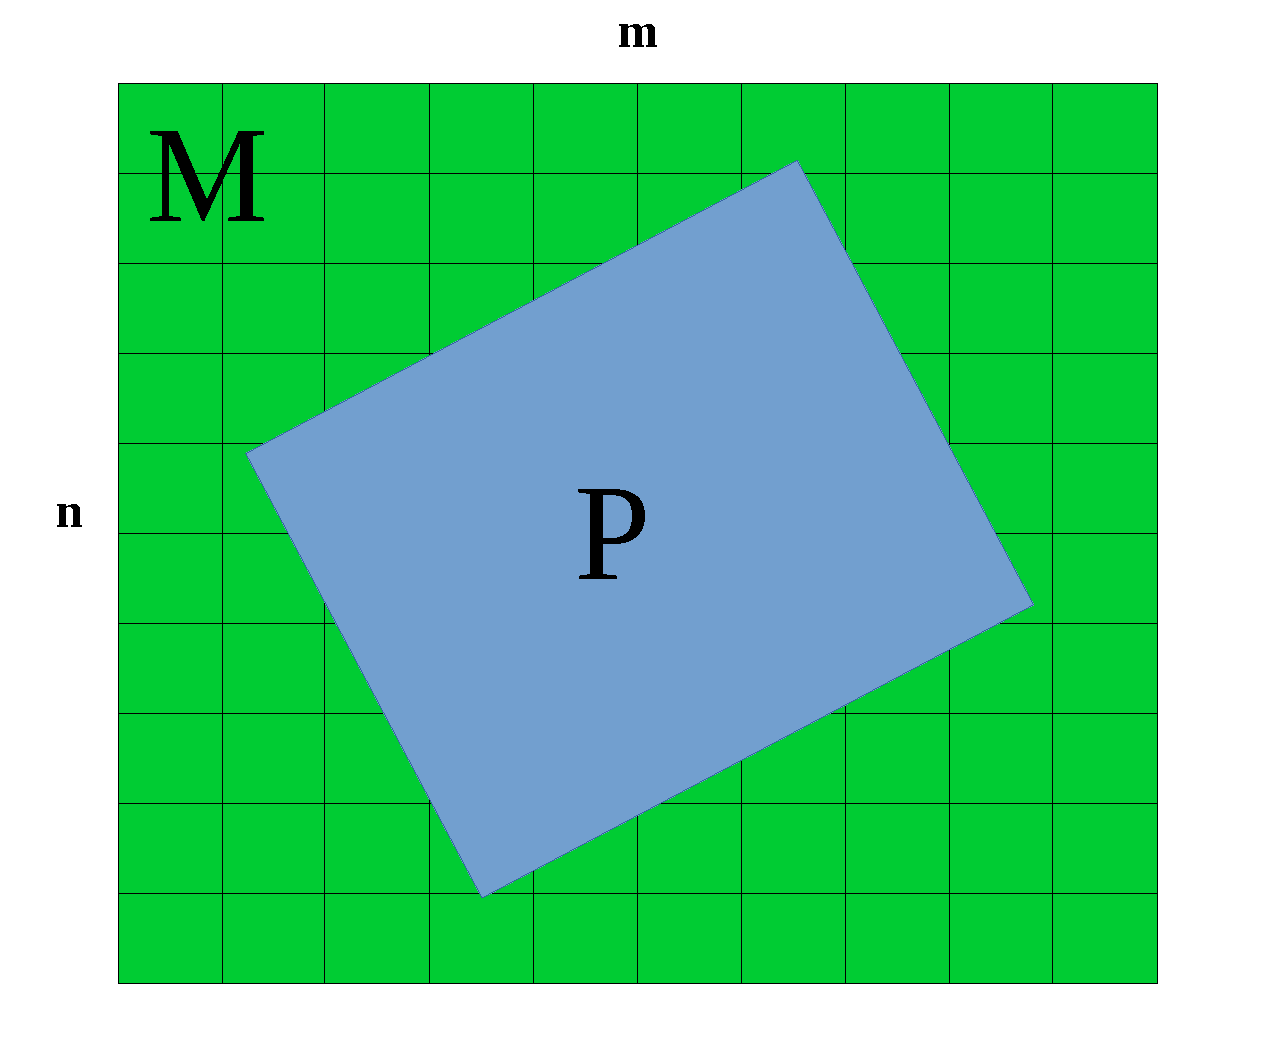
\includegraphics[ clip, scale=0.5]{mandf}}
%	\centering
%	\caption{blah}
%	\label{fig:matrix_m}
%\end{figure}
Załóżmy, że $p(x,y)$ jest funkcją mówiącą o tym czy punkt o współrzędnych $(x, y)$ znajduje się wewnątrz $P$. Jeśli $p = 0$ punkt należy do $P$, w przeciwnym wypadku $p=1$. Zraszacz jest definiowany jako okrąg reprezentowany przez promień $r_{i}$, współrzędne środka $(x_i, y_i)$ oraz konkretny model $t_{i}$. Środek każdego zraszacza musi zawierać się w $P$, czyli $p(x_{i}, y_{i}) = 0$.\\
Kwadrat o współrzędnych $(x,y)$ jest nawodniony jeśli znajduje się w zasięgu zraszacza. Jest to wyrażone następującą funkcją:
\begin{equation}
	is\_irr(x, y, s_{i}) = \begin{cases}
							1,& \text{jeśli } (x - x_{i})^{2} + (y - y_{i})^2 \leq r_{i}^{2}\\
							0,& w.p.p
						  \end{cases}
\end{equation}
, gdzie $x$ oraz $y$ oznaczają współrzędne środka kwadratu; $s_{i}$ jest konkretnym zraszaczem; $x_{i}, y_{i}$ oznaczają współrzędne zraszacza $s_{i}$; $r_{i}$ jest liczba wyrażającą zasięg zraszacza.\\\\
Załóżmy, że $S$ jest zbiorem wszystkich rozmieszczonych zraszaczy. Wtedy dany kwadrat jest nawodniony jeśli znajduje się w zasięgu przynajmniej jednego zraszacza ze zbioru $S$:
\begin{equation}
	irr(x, y, S) = \begin{cases}
				   	1,& \text{jeśli } \sum_{i=1}^{S} is\_irr(x,y,s_{i}) > 0 \\
				   	0,& w.p.p			   	
				   \end{cases}
\end{equation}
Generalnie poprzez stopień nawodnienia danego obszaru rozumie się różnicę pomiędzy liczbą wszystkich elementów macierzy $M$ należących do $P$, a liczbą nawodnionych elementów tej macierzy należących do $P$:
\begin{equation}\label{eq:simple_f1}
	F_{0}(S) = \sum_{m=1}^{M}\sum_{n=1}^{N} p(m,n) \cdot (1 - irr(m,n,S))
\end{equation}
Im wartość funkcji $F_{0}$ jest mniejsza tym mniej jest obszarów nienawodnionych, a więc rozwiązanie jest lepsze. $F_{0} = $ jest rozwiązaniem idealnym z perspektywy kryterium nawodnienia.\\\\
Jak zostało wspomniane w poprzednich rozdziałach zaimplementowane algorytmy oceniają stopień nawodnienia obszaru na dwa sposoby w zależności od tego czy wybrana jest opcja minimalizacji nawodnienia poza wskazanym obszarem. Jeśli minimalizacja jest wyłączona do obliczeń używana jest prosta funkcja opisana powyżej \eqref{eq:simple_f1}. Bardziej szczegółowe rozwinięcie funkcji przewiduje wprowadzenie kary za naruszenie ograniczeń:

\begin{equation}
\begin{split}
	F_{1}(S) = \sum_{m=1}^{M}\sum_{n=1}^{N} p(m,n) \cdot (1 - irr(m,n,S)) \\ + 
	\alpha \cdot \bigg{[}\dfrac{\sum_{m=1}^{M}\sum_{n=1}^{N} (1 - p(m,n)) \cdot irr(m,n,S) \cdot 100}{\sum_{m=1}^{M}\sum_{n=1}^{N} p(m,n)} \\ + \dfrac{\sum_{m=1}^{M}\sum_{n=1}^{N} p(m,n) \cdot ovrirr(m,n,S) \cdot 100}{\sum_{m=1}^{M}\sum_{n=1}^{N} p(m,n)}\bigg{]}
\end{split}
\end{equation}
, gdzie $\alpha$ jest zmienną określającą to czy na funkcję celu wpływa minimalizacja nawodnienia poza wskazanym obszarem. Zmienna $\alpha$ może przyjmować wartość 0 lub 1. Jeśli $\alpha=1$ minimalizacja jest brana pod uwagę; $ovrirr(m,n,S)$ jest funkcją mówiącą czy dany obszar został nadmiernie nawodniony \eqref{eq:is_overirrigated_func}.
\begin{equation}\label{eq:is_overirrigated_func}
	ovrirr(x,y,S) = \begin{cases}
				1,& \text{jeśli } \sum_{i=1}^{S} is\_irr(x,y,s_{i}) > 1 \\
				0,& w.p.p
			   \end{cases}
\end{equation}
\\Jak zostało wspomniane wcześniej, każdy rozmieszczony zraszacz charakteryzowany jest przez konkretny model. Załóżmy, że $C(t_{i})$ jest funkcją zwracającą cenę rynkową dla danego modelu $t_i$. Wtedy całkowity koszt konkretnego rozwiązania wynosi:
\begin{equation}
	F_{2}(S) = \sum_{i=1}^{S} C(t_{i})
\end{equation}\\
Podsumowując celem zadania jest rozwiązanie następującego problemu optymalizacyjnego:

\begin{equation}
	\begin{split}
		min \text{  } & 	F_{1}(S) = \sum_{m=1}^{M}\sum_{n=1}^{N} p(m,n) \cdot (1 - irr(m,n,S)) \\ +& 
		\alpha \cdot \bigg{[}\dfrac{\sum_{m=1}^{M}\sum_{n=1}^{N} (1 - p(m,n)) \cdot irr(m,n,S) \cdot 100}{\sum_{m=1}^{M}\sum_{n=1}^{N} p(m,n)} \\ +& \dfrac{\sum_{m=1}^{M}\sum_{n=1}^{N} p(m,n) \cdot ovrirr(m,n,S) \cdot 100}{\sum_{m=1}^{M}\sum_{n=1}^{N} p(m,n)}\bigg{]}\\\\
		min \text{  }&	F_{2}(S) = \sum_{i=1}^{S} C(t_{i})
	\end{split}
\end{equation}

\subsection{Porównanie algorytmów genetycznych}
\subsubsection{Plan badań}
Złożoność oceny algorytmów służących do optymalizacji wielokryterialnej jest znacznie większa niż tej dla algorytmów rozwiązujących problemy obejmujące jedno kryterium. Wynika tak z samej definicji rozwiązania problemu wielokryterialnego, która wyjaśniona została wcześniej. Oceniając rozwiązanie takiego problemu należy wziąć pod uwagę następujące składowe:
\begin{itemize}
	\item Dystans znalezionego niezdominowanego zbioru rozwiązań od prawdziwego zbioru Pareto
	\item Równomierny rozkład znalezionych rozwiązań
	\item Długość przedziału pokrytego przez znalezione rozwiązania
	\item Czas wykonania algorytmu\\
\end{itemize}
Na potrzeby analizy i oceny dwóch zaproponowanych algorytmów wybrane zostały cztery metryki:
\begin{enumerate}
	\item \textit{Współczynnik błędu (ER):} wskazuje procent rozwiązań, które nie należą do prawdziwego zbioru Pareto.
	\begin{equation}
		ER = \dfrac{\sum_{i=1}^{n} e_{i}}{n}
	\end{equation}
	Gdzie $n$ jest liczbą znalezionych niezdominowanych rozwiązań; $e_{i}$ zmienną określającą czy dane rozwiązanie znajduje się w prawdziwym zbiorze Pareto. Jeśli $e_{i} = 0$ rozwiązanie znajduje się w prawdziwym zbiorze Pareto, w przeciwnym razie $e_{i} = 1$. $ER = 0$ oznacza idealne rozwiązanie.\\
	\item \textit{Równomierny rozkład (SP):} metoda mierząca wariancję dystansu sąsiadujących rozwiązań znajdujących się na znalezionym froncie Pareto.
	\begin{equation}
		SP = \sqrt{\dfrac{1}{n-1}\sum_{i=1}^{n}{(\overline{d} - d_{i})}^{2}}
	\end{equation}
	Gdzie $n$ jest liczbą znalezionych niezdominowanych rozwiązań; $d_{i}$ oznacza dystans Euklidesowy pomiędzy danym rozwiązaniem, a jego najbliższym sąsiadem; $\overline{d}$ jest wartością oznaczającą średni dystans pomiędzy rozwiązaniami. Wartość $SP = 0$ oznacza, że znalezione rozwiązania są rozłożone równomiernie.\\
	\item \textit{Jakość ogólna (DG):}  wskazuje jak daleko od prawdziwego zbioru Pareto znajduje się zbiór znalezionych niezdominowanych rozwiązań. Miara zdefiniowana w następujący sposób:
	\begin{equation}
		DG = \dfrac{\sqrt{\sum_{i=1}^{n} d_{i}^{2}}}{n}
	\end{equation}
	Gdzie $n$ oznacza liczbę znalezionych niezdominowanych rozwiązań; $d_{i}$ jest dystansem Euklidesowym pomiędzy danym rozwiązaniem, a najbliższym rozwiązaniem należącym do prawdziwego frontu Pareto. Wartość $DG = 0$ oznacza, że wszystkie znalezione rozwiązania leżą na prawdziwym froncie Pareto.\\
	\item \textit{Długość frontu (FE):} metoda wskazująca jak duży obszar jest pokryty przez znalezione niezdominowane rozwiązania.
	\begin{equation}
		FE = \sum_{k=1}^{K} \max_{i, j!=i} \sqrt{(f_{i}^{k} - f_{j}^{k})^{2}}
	\end{equation}
	Gdzie $K$ oznacza liczbę funkcji celu; $f_{i}^{k}$ jest wartością $i$-tego rozwiązania z perspektywy kryterium $k$.\\
\end{enumerate}
Aby skorzystać z powyższych metryk konieczne jest znalezienie prawdziwego frontu Pareto. Na potrzeby badań został on wygenerowany   poprzez wybranie niezdominowanych rozwiązań ze skumulowanej puli rozwiązań powstałej na wskutek uruchomienia symulacji 10 razy dla każdego algorytmu. Rezultaty każdej symulacji były dodawane do puli po czym zredukowane do rozwiązań niezdominowanych.\\
Dla badań przygotowanych zostało 6 przypadków testowych. Zostały one podzielone ze względu na wielkość obszaru mającego zostać nawodniony oraz tego czy algorytm ma minimalizować nawadnianie poza zaznaczonym obszarem. Kształt wybranych obszarów został dobrany tak, aby jak najlepiej wizualizować wpływ ograniczeń na działanie algorytmów.

\begin{table}[]
\centering
\caption{Przypadki testowe}
\label{my-label}
\begin{tabular}{|l|l|}
\hline
Wielkość & Obszar \\ \hline
Mały & 1 \\ \hline
Średni & 2 \\ \hline
Duży & 3 \\ \hline
\end{tabular}
\end{table}

\subsubsection{Rezultaty badań}
\subsubsection{Podsumowanie badań}

\chapter{Podsumowanie}

\begin{mydef}
\textbf{Definicja} - pierwsza
\end{mydef}




 \clearpage
\appendix
\chapter{Appendix 1}


\clearpage
\pagestyle{plain}
\listofmyfigure
\listofmyequations
\listofmyalgorithm
\clearpage

%\bibliographystyle{apalike}%Used BibTeX style is unsrt

\bibliographystyle{iisthesis}
\bibliography{bibliography}

\end{document}

